%!TEX root = ../slides.tex
\section{Solution}
{\aauwavesbg%
\begin{frame}[plain]
  \begin{textblock*}{8.5cm}(4.3cm,8.3cm)
  \small
  \textbf{Architecture of proposed system solution. The global perception-action cycle, the different memory types, and the internal feedback loops are observed.}
  \end{textblock*}

  \begin{textblock*}{1cm}(12cm,9.3cm)
  \scriptsize
  \insertframenumber~/~\inserttotalframenumber
  \end{textblock*}

  \centering
  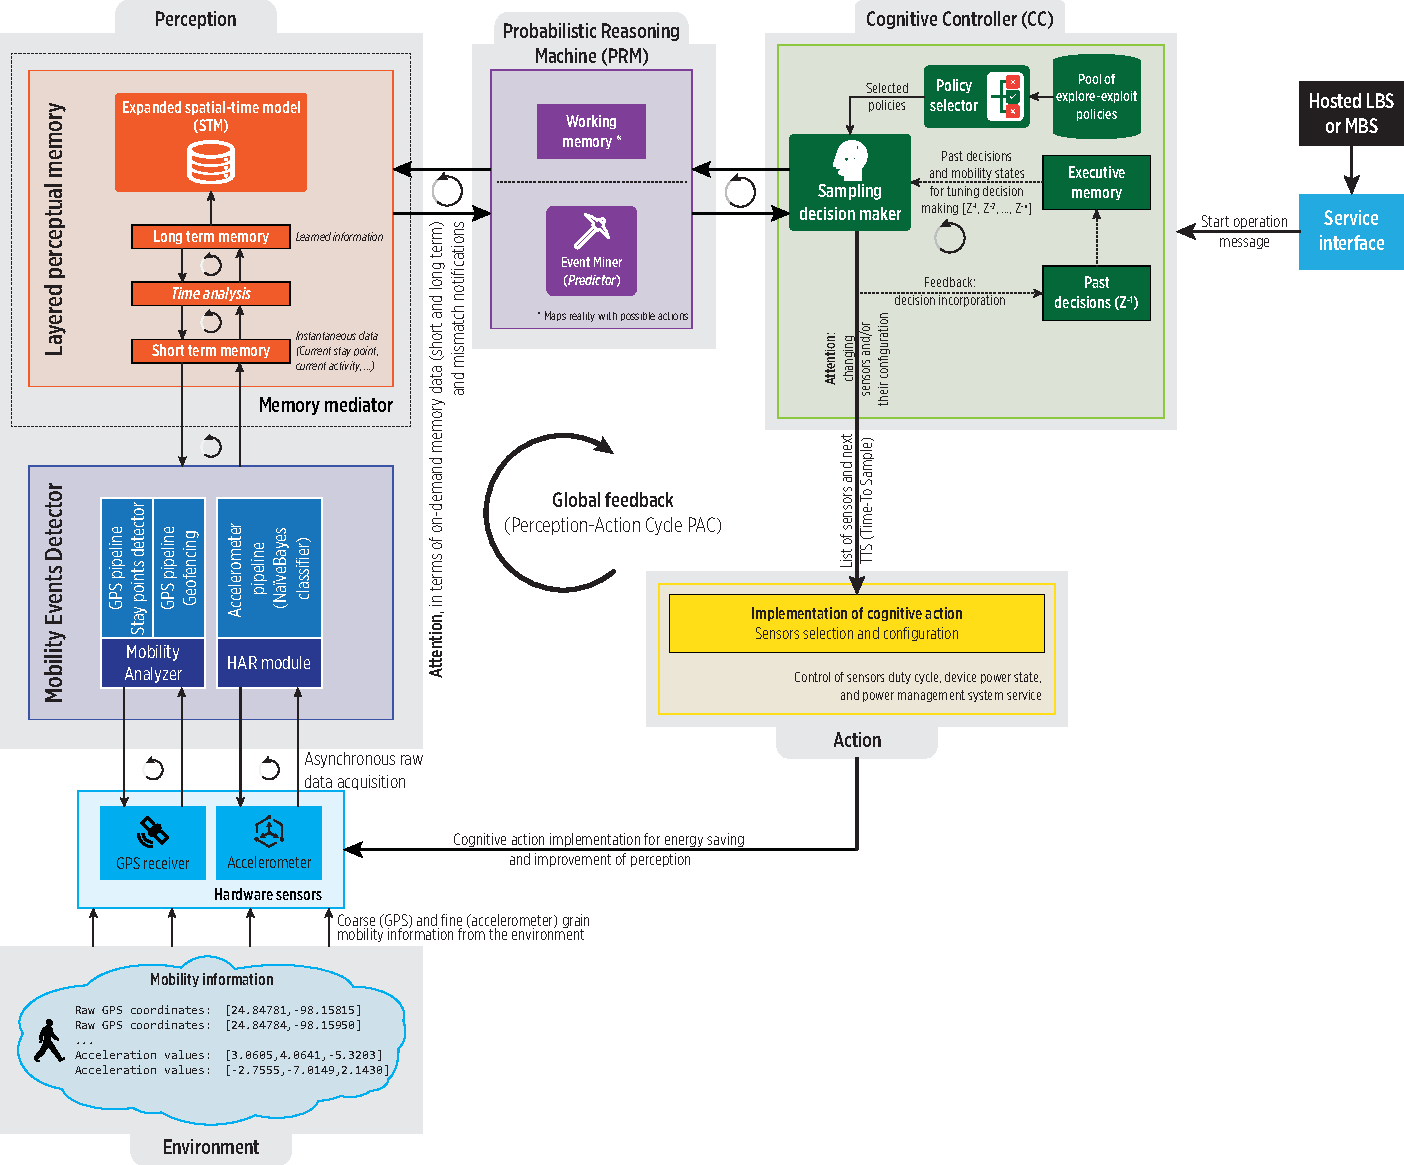
\includegraphics[width=0.98\textwidth]{vectors/inspired-cds-solution-for-slides}
\end{frame}}
    

\subsection{Perception components}
\begin{frame}{Perception components}{Mobility Events Detector}
\small
\begin{figure}
    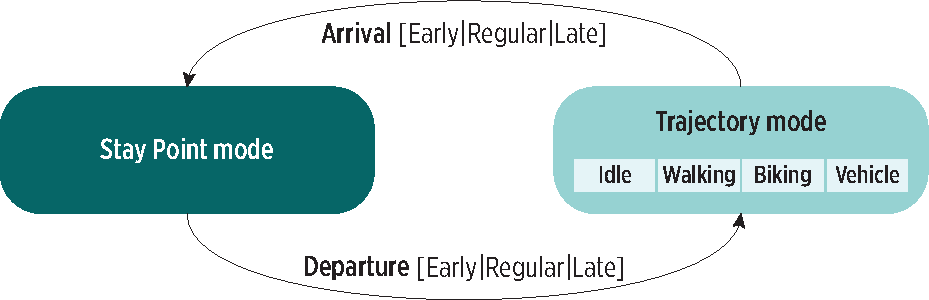
\includegraphics[width=0.55\textwidth]{vectors/mobility-as-events}
    \caption{Individual's mobility as a sequence of high level states and associated events detected from raw sensor data~\cite{Alessandretti2017,Wang2014}.}
\end{figure}

\begin{block}{\small \textbf{Mobility Events Detector}} 
Aimed at identifying:
\begin{itemize}
    \item Coarse-grain mobility events.
    \item Fine-grain mobility events.
\end{itemize}
\end{block}
\end{frame}

\begin{frame}{Perception components}{Mobility Events Detector: \emph{Stay Points Detector} module}
\small
\vspace{-0.3cm}
\begin{columns}
\begin{column}[T]{0.5\textwidth}
\begin{block}{\small \emph{\textbf{Stay Points Detector}} module}
{
  \centering
  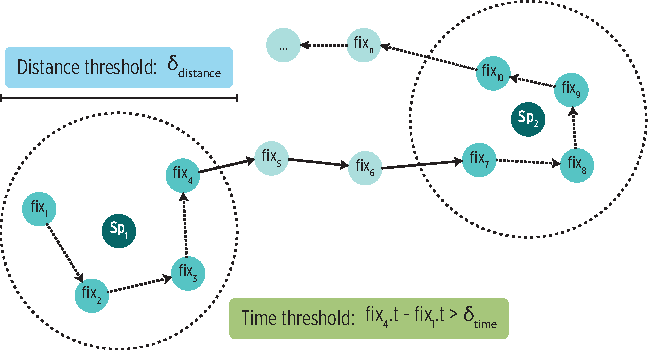
\includegraphics[width=0.75\textwidth]{vectors/zhen-algorithm-behavior}
  \captionof{figure}{A conceptual representation of the stay points detection algorithm behavior.}
}
\end{block}
\end{column}

\begin{column}[T]{0.5\textwidth}
\begin{block}{\small \emph{\textbf{Geofencing}} module}
{
  \centering
  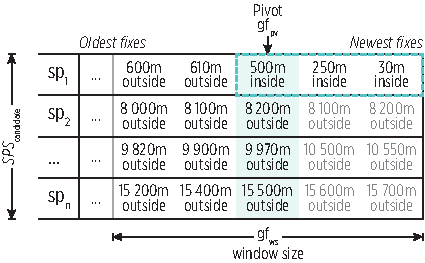
\includegraphics[width=0.65\textwidth]{vectors/geofencing-window-based-snapshot-for-slides}
  \captionof{figure}{A conceptual representation of the window-based geofencing operation.}
}
\end{block}
\end{column}
\end{columns}

\begin{block}{\small \emph{\textbf{HAR}} module}
{
  \centering
  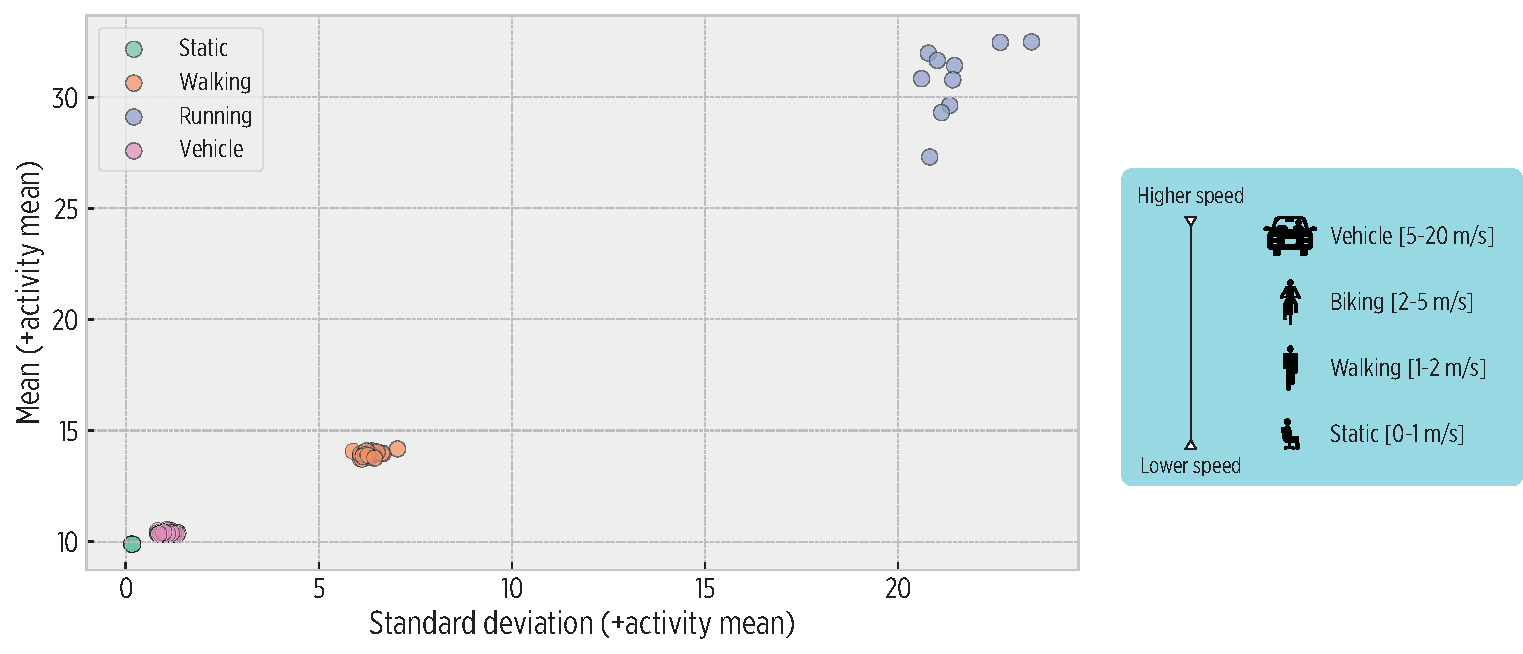
\includegraphics[width=0.6\textwidth]{vectors/har-patterns-for-slides-v2}
  \captionof{figure}{Distribution of mean and standard deviation features employed by the NaïveBayes classifier of the HAR module.}
}
\end{block}
\end{frame}


\begin{frame}{Layered perceptual memory}{Short and long-term memory information}
\vspace{-0.25cm}
\small
\begin{block}{\small \textbf{Layered perceptual memory}}
\begin{itemize}
    \item Short-term memory information: current (observed) mobility status.
    \item Long-term memory information: the Expanded Spatial-Time model (STM).
\end{itemize}
\end{block}

\begin{block}{\small \textbf{Expanded Spatial-Time model}}
\begin{itemize}
  \item The highest level of mobility information held by the system.
\end{itemize}
{
  \centering
  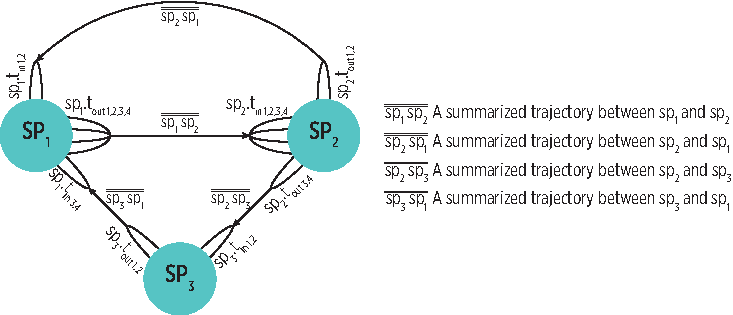
\includegraphics[width=0.7\textwidth]{vectors/stm-slides}
  \captionof{figure}{A conceptual representation of the STM's structure.}
\par }
\end{block}
\end{frame}

\begin{frame}{Layered perceptual memory}{Expanded Spatial-Time model (STM)}
\small
\begin{block}{\small \textbf{Generation of the STM}}
\begin{itemize}
    \item Incrementally built with the coarse-grain mobility events detected by the \emph{Mobility Events Detector}.
\end{itemize}
{
  \centering
  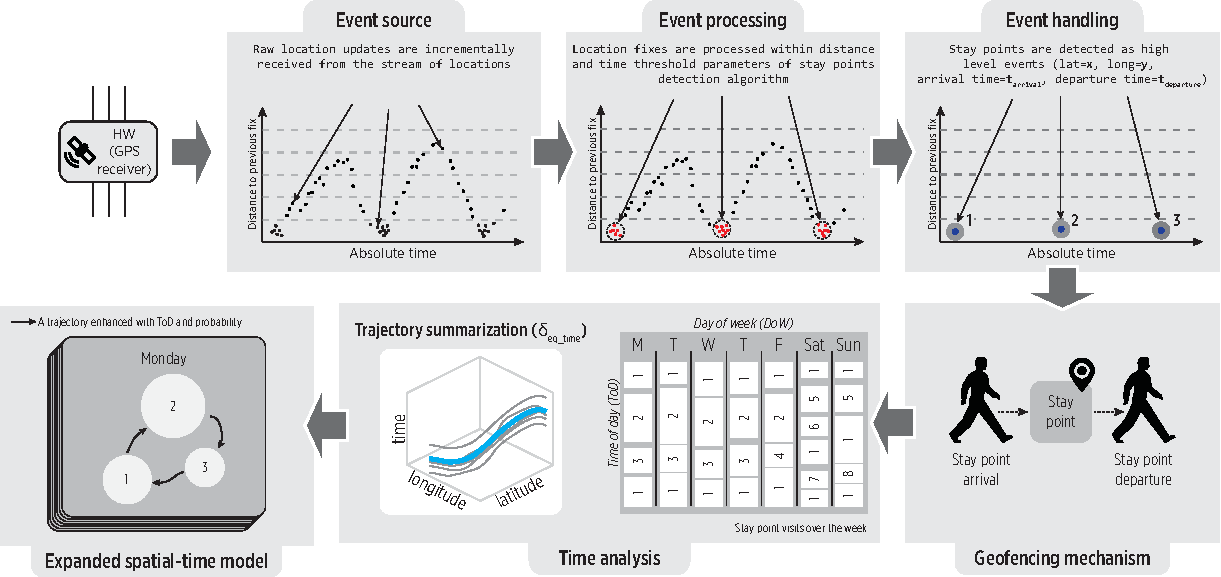
\includegraphics[width=\textwidth]{vectors/event-driven-memory-generation-for-slides}
  \captionof{figure}{A conceptual representation of the steps for generating the STM from raw sensors data.}
  \par
}
\end{block}
\end{frame}

\subsection{Working memory}
\begin{frame}{Probabilistic Reasoning Machine (PRM)}{Working memory}
\small
\begin{block}{\small \textbf{PRM features}}
\begin{itemize}
    \item It gives a meaning to the observed mobility information with respect of the STM information.
    \item It produces an estimation of future mobility state that links perceptual and working memory.
\end{itemize}
\end{block}

\begin{block}{\small \textbf{Interpretation}}
\begin{itemize}
  \item The \emph{Event Miner} traverses the \textbf{STM} for identifying whether learned information is:
  \begin{itemize}
     \item Consistent, or
     \item Inconsistent (mismatch)
   \end{itemize}
   with respect of observed mobility information.
\end{itemize}
\end{block}

\begin{block}{\small \textbf{Estimation}}
\begin{itemize}
\item The \emph{Event Miner} looks in the \textbf{STM} for a link (if any) with learned mobility information for generating spatial-time estimations:
\begin{itemize}
  \item Get next departure time.
  \item Get next arrival time.
\end{itemize}
\end{itemize}
\end{block}

\end{frame}

\subsection{Cognitive controller}
\begin{frame}{Cognitive controller (CC)}{Description}
\small
\vspace{-0.5cm}
\begin{columns}
\begin{column}[T]{0.5\textwidth}
\begin{block}{\small \textbf{Goals}}
  \begin{itemize}
      \item To reduce the energy consumption of location tracking by relying on PRM's estimations.
      \item To reduce the system uncertainty about current user mobility.
  \end{itemize}
\end{block}
\end{column}

\begin{column}[T]{0.5\textwidth}
\begin{block}{\small \textbf{Possible cognitive actions}}
  \begin{itemize}
    \item \textbf{Exploitation policies}: When system uncertainty is low for saving energy purposes.
    \item \textbf{Exploration policies}: When system uncertainty is high for recovering for accuracy loss.
  \end{itemize}
\end{block}
\end{column}
\end{columns}

\begin{figure}
  \centering
  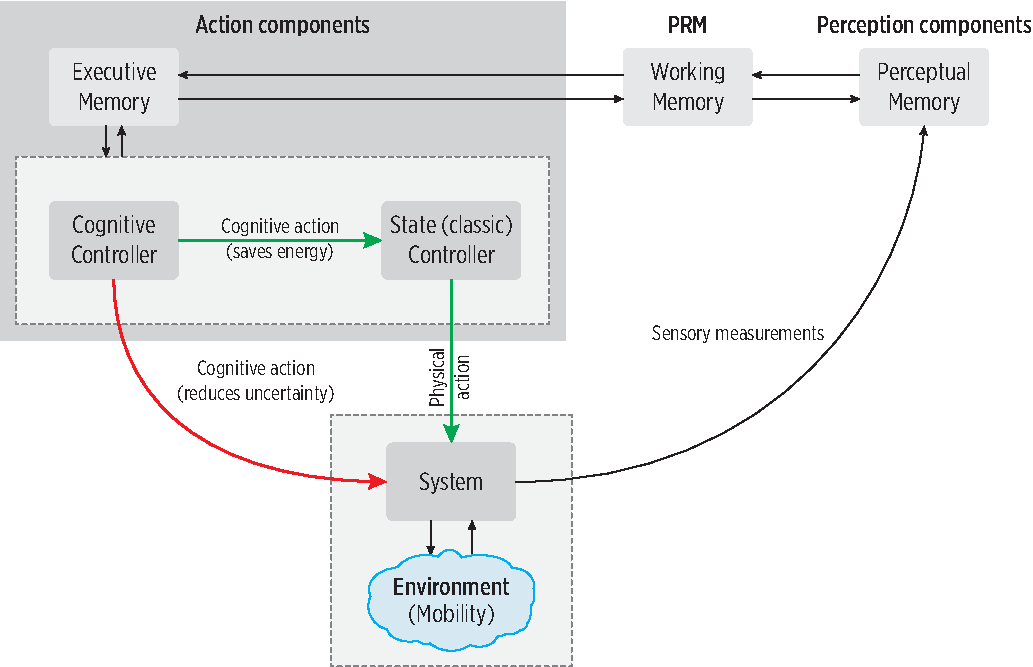
\includegraphics[width=0.65\textwidth]{vectors/cognitive-controller-architecture}
  \caption{A generic architecture for a cognitive controller.}
\end{figure}

\end{frame}

\begin{frame}{Cognitive controller}{Policies tailored for user mobility}
\small
\vspace{-0.3cm}
\begin{block}{\small \textbf{Stay point mode}}
\begin{columns}
\begin{column}{0.45\textwidth}
{
  \centering
  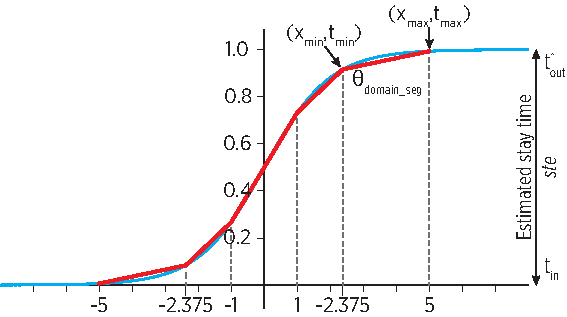
\includegraphics[width=0.75\linewidth]{vectors/sigmoid-segmentation-for-slides}
  \captionof{figure}{Approximation of the sigmoid through straight segments.}
}
\end{column}

\begin{column}{0.55\textwidth}
{
  \centering
  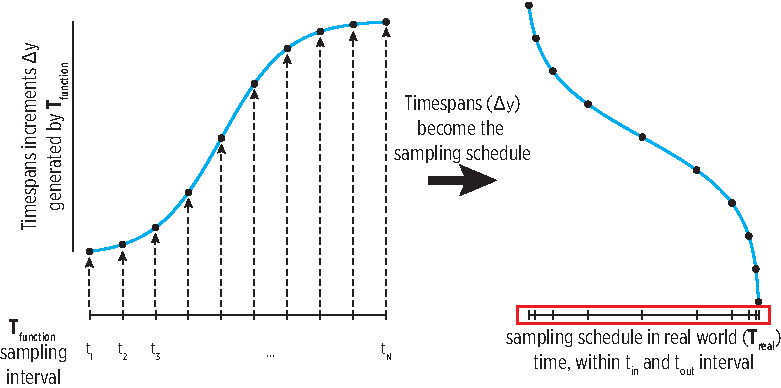
\includegraphics[width=0.80\linewidth]{vectors/sigmoid-driven-sampling-policy-for-slides}
  \captionof{figure}{A snapshot of the process for producing a sigmoid sampling.}
}
\end{column}
\end{columns}
\end{block}

\begin{block}{\small \textbf{Trajectory mode}}
{
  \centering
  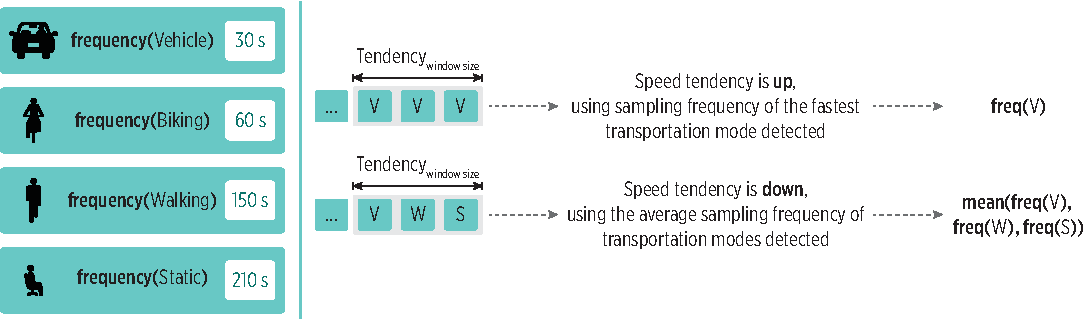
\includegraphics[width=0.7\linewidth]{vectors/trajectory-sampling}
  \captionof{figure}{GPS sampling adaptation during trajectory based on the speed tendency of detected transportation modes.}
}
\end{block}
\end{frame}


\begin{frame}{Cognitive controller}{\emph{Sampling Decision Maker} module}
\small
\vspace{-0.3cm}
\begin{block}{\small \textbf{Sampling Decision Maker module}}
  \begin{itemize}
      \item It filters from the \emph{pool of exploration-exploitation policies} those apt for the mobility state detected by PRM.
      \item It updates its \emph{Executive Memory} with the selected cognitive action for feedback in further executions.
  \end{itemize}
\end{block}

\begin{block}{\small \textbf{Implementation of cognitive action}}
{
  \centering
  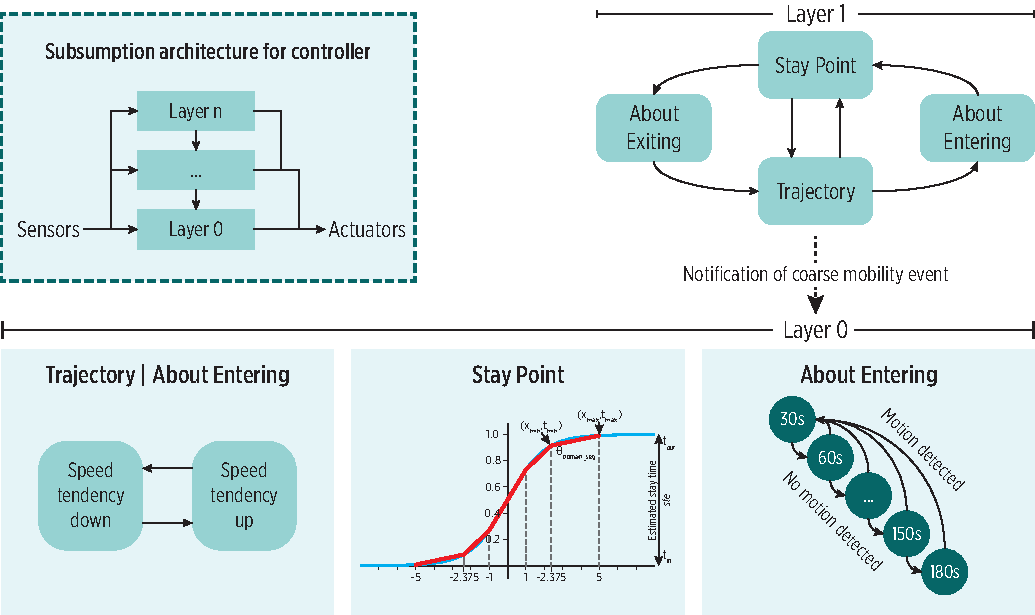
\includegraphics[width=0.65\linewidth]{vectors/brooks-inspired-controller}
  \captionof{figure}{The subsumption architecture of the controller and the reactions for different coarse grain mobility events.}
}
\end{block}
\end{frame}
